\section{Project requirements}
%%%%%%%%%%%%%%%%%%%%%%%%%%%%%%%%%%%%%%%%%%%%%%%%%%%%%%%%%%%%%%%%%%%%%%%%%%%%%%%%
% Introduction.
% What the project requirements are.
%%%%%%%%%%%%%%%%%%%%%%%%%%%%%%%%%%%%%%%%%%%%%%%%%%%%%%%%%%%%%%%%%%%%%%%%%%%%%%%%

Before development can take place the team responsible for a project collects the necessary requirements for a project and criteria for success.
These are what the client ought to ``grade'' the final product against to judge ``Was this project a success?''

\subsection{Preliminary project requirements}
%%%%%%%%%%%%%%%%%%%%%%%%%%%%%%%%%%%%%%%%%%%%%%%%%%%%%%%%%%%%%%%%%%%%%%%%%%%%%%%%
% Your original Requirements Document.

% > This needs to be the original document, showing what you thought, at the time, was the project definition.
% > This needs to include the original Gantt chart.
%%%%%%%%%%%%%%%%%%%%%%%%%%%%%%%%%%%%%%%%%%%%%%%%%%%%%%%%%%%%%%%%%%%%%%%%%%%%%%%%
\subsubsection{Introduction}

\paragraph{Purpose}
%%%%%%%%%%%%%%%%%%%%%%%%%%%%%%%%%%%%%%%%%%%%%%%%%%%%%%%%%%%%%%%%%%%%%%%%%%%%%%%%
% Delineate the purpose of the SRS
% Specify the intended audience of the SRS
%%%%%%%%%%%%%%%%%%%%%%%%%%%%%%%%%%%%%%%%%%%%%%%%%%%%%%%%%%%%%%%%%%%%%%%%%%%%%%%%

This document is intended to present a detailed description of the high performance XML/XSLT transformation server being developed by the Oregon State University CS Capstone Team ``XZES40''.
The intended audience for this document are the developers and sponsors of the project.

% The purpose of this document is to present a detailed description of high performance XML/XSLT transformation server.
% This document is intended for people who maintain server and the developers of the system.

\paragraph{Scope}
%%%%%%%%%%%%%%%%%%%%%%%%%%%%%%%%%%%%%%%%%%%%%%%%%%%%%%%%%%%%%%%%%%%%%%%%%%%%%%%%
% 1. Identify the software product(s) to be produced by name (e.g., Host DBMS, Report Generator, etc.);
% 2. Explain what the software product(s) will, and, if necessary, will not do;
% 3. Describe the application of the software being specified, including relevant benefits, objectives, and goals;
% 4. Be consistent with similar statements in higher-level specifications (e.g., the system requirements specification), if they exist.
%%%%%%%%%%%%%%%%%%%%%%%%%%%%%%%%%%%%%%%%%%%%%%%%%%%%%%%%%%%%%%%%%%%%%%%%%%%%%%%%

The name of this software, for lack of a better one, will be XZES40-Transformer.

The core product being delivered is a high performance XML/XSLT transformation server.
This server will be able to perform repetitive document transformations quickly and efficiently by caching previously processed and compiled documents.
Time is saved by pulling from an in-memory cache of documents and their compiled state rather than downloading and compiling documents which have already been processed, as current systems tend to do.
XZES40-Transformer will also carry out transformations in parallel.
It will transfer documents to and from clients via the HTTP or HTTPS protocol.

The target platform for XZES40-Transformer will be Debian Linux 8 (``Jessie'').
The core product will be designed to allow the program to be ported easily from Linux to other operating systems like Windows and BSD.

In addition to the core server there will also be a command-line interface and web-interface developed to interact with the application, these will be called XZES-CLI and XZES-Web respectively.

% This software system will create a high performance XML/XSLT transformation server that can perform repetitive document transformations in a high-volume environment.
% XSLT is used to convert an XML document to another XML document, or other types of documents that can be recognized by the browser, such as HTML and XHTML.
% In normal, XSLT accomplishes this by converting each XML element to an (X)HTML element.
% With XSLT, you can add or remove elements and attributes from or to the output file.
% You can also rearrange elements, perform tests, and decide which elements to hide or display.

\paragraph{Definitions, acronyms, and abbreviations}
%%%%%%%%%%%%%%%%%%%%%%%%%%%%%%%%%%%%%%%%%%%%%%%%%%%%%%%%%%%%%%%%%%%%%%%%%%%%%%%%
% Provide the definitions of all terms, acronyms, and abbreviations required to properly interpret the SRS.
% This information may be provided by reference to one or more appendixes in the SRS or by reference to other documents.
%%%%%%%%%%%%%%%%%%%%%%%%%%%%%%%%%%%%%%%%%%%%%%%%%%%%%%%%%%%%%%%%%%%%%%%%%%%%%%%%

Below is a list of acronyms and abbreviations used throughout the document:

\begin{itemize}
  \item Extensible Markup Language XML: The human-readable data format used and processed by our application.
  \item Extensible Stylesheet Markup Language (XSLT): The human-readable format used to transform documents in our application.
  \item Xerces-C \cite{xerces}: One library used to perform XML transformation in C.
  \item Xalan-C \cite{xalan}: One library used to XML transformation in C.
  \item ICU \cite{icu}: One library used to process UTF-8 character formated documents.
  \item Hypertext Transfer Procol (HTTP/HTTPS): The protocol over which XZES40-Transformer will interact with remote clients.
  \item HTTP Application Programming Interface (HTTP API): A standard way of communicating with a web application.
  \item Unified Resource Locator / Identifier (URL/URI): Addressable location of a resource over the internet (e.g., a website address).
  \item Debian 8 (``Jessie''): The target Linux-based operating system XZES40-Transformer will run on.
  \item Unicode Transmission Format 8 (UTF-8): The international standard for encoding text-based data.
  \item Apache Web-server: A Free and Open Source web-server.
  \item Common Gateway Interface Script (CGI Script): Server-side scripts that can run applications on client's behalf.
\end{itemize}
% XML is a simple and standard way of exchanging raw data between computer programs.
% It is not only easy to be written and read but also solve the application of information exchange between systems.
% There are two basic needs:
% 
% \begin{enumerate}
%   \item Separate the data from the representation
%   \item Transfer data between different applications
% \end{enumerate}
% 
% In order to make the data easy for people to read and understand, we need to display information or pint out.
% For example, the data into an HTML file, a PDF file, or even a sound.
% Similarly, in order to adapt the data to different applications, a data format is converted to another data format, such as the demand format may be a text file, a SQL statement and an HTTP message.
% XSLT is used to achieve this conversion function of the language.
% XML is converted to HTML, XSLT is the most important function.
% XSLT: Extensible Stylesheet Language Transformations
% XML: Extensible Markup Language


\subsubsection{Overall description}

%%%%%%%%%%%%%%%%%%%%%%%%%%%%%%%%%%%%%%%%%%%%%%%%%%%%%%%%%%%%%%%%%%%%%%%%%%%%%%%%
% This section of the SRS should describe the general factors that affect the product and its requirements.
% This section does not state specific requirements.
% Instead, it provides a background for those requirements, which are defined in detail in Section 3 of the SRS, and makes them easier to understand.
%%%%%%%%%%%%%%%%%%%%%%%%%%%%%%%%%%%%%%%%%%%%%%%%%%%%%%%%%%%%%%%%%%%%%%%%%%%%%%%%

The following sections of this document outline the factors that affect the creation of XZES40-Transformer at a high-level.

\paragraph{Product perspective}
%%%%%%%%%%%%%%%%%%%%%%%%%%%%%%%%%%%%%%%%%%%%%%%%%%%%%%%%%%%%%%%%%%%%%%%%%%%%%%%%
% This paragraph of the SRS should put the product into perspective with other related products.
% If the product is independent and totally self-contained, it should be so stated here.
% If the SRS defines a product that is a component of a larger system, as frequently occurs,
% then this paragraph should relate the requirements of that larger system to functionality of the software and should identify interfaces between that system and the software.
% A block diagram showing the major components of the larger system, interconnections, and external interfaces can be helpful.
% This paragraph should also describe how the software operates inside various constraints.
% For example, these constraints could include
% 1. System interfaces;
% 2. User interfaces;
% 3. Hardware interfaces;
% 4. Software interfaces;
% 5. Communications interfaces;
% 6. Memory;
% 7. Operations;
% 8. Site adaptation requirements.
%%%%%%%%%%%%%%%%%%%%%%%%%%%%%%%%%%%%%%%%%%%%%%%%%%%%%%%%%%%%%%%%%%%%%%%%%%%%%%%%

\textbf{System interfaces}
%%%%%%%%%%%%%%%%%%%%%%%%%%%%%%%%%%%%%%%%%%%%%%%%%%%%%%%%%%%%%%%%%%%%%%%%%%%%%%%%
% This should list each system interface and identify the functionality of the software to accomplish the system requirement and the interface description to match the system.
%%%%%%%%%%%%%%%%%%%%%%%%%%%%%%%%%%%%%%%%%%%%%%%%%%%%%%%%%%%%%%%%%%%%%%%%%%%%%%%%

The XZES40-Transformer application will interface with the outside world over the internet via the HTTP networking protocol.
The application will recieve HTTP POST requests to the application URI endpoint containing the documents to be transformed.
Once the transformation is completed the transformed document will be sent to the user for download.

In addition to the transformed file the application will respond with an HTTP \textbf{OK} status.
If an error occurs it will respond with a \textbf{SERVER ERROR} status and no file.

% \begin{enumerate}
%   \item Data base
%   \item User and manager
%   \item XML servers
% \end{enumerate}
%
% Our server has 3 layer of actor, first layer is user part, such as reader and manager.
% Second layer is XML servers, which contain XML parse and other XML transformation part.
% Third layer is our database where we store our data.
% User can connect to webpage and send request to XML servers,and then XML servers will search from database and query data out, after that XML server can compile to Unicode type file and give back to user.

\textbf{User interfaces}
%%%%%%%%%%%%%%%%%%%%%%%%%%%%%%%%%%%%%%%%%%%%%%%%%%%%%%%%%%%%%%%%%%%%%%%%%%%%%%%%
% This should specify 
% 1. The logical characteristics of each interface between the software product and its users.
%    This includes those configuration characteristics (e.g., required screen formats, page or window layouts, 
%    content of any reports or menus, or availability of programmable function keys) necessary to accomplish the software requirements.
% 2. All the aspects of optimizing the interface with the person who must use the system.
%    This may simply comprise a list of do's and don'ts on how the system will appear to the user.
%    One example may be a requirement for the option of long or short error messages.
%    Like all others, these requirements should be verifiable, e.g., “a clerk typist grade 4 can do function X in Z min after 1 h of training” rather than “a typist can do function X.” (This may also be specified in the Software System Attributes under a section titled Ease of Use.)
%%%%%%%%%%%%%%%%%%%%%%%%%%%%%%%%%%%%%%%%%%%%%%%%%%%%%%%%%%%%%%%%%%%%%%%%%%%%%%%%

XZES40 will have two user interfaces which will access it's functionality over the internet.

\begin{itemize}
    \item {
      A Website to access XZES40-Transformer via a web-browser.
      This interface will be called ``XZES40-Web''.
    }
    \item {
      A CLI to access XZES40-Transformer via a terminal interface.
      This interface will be called ``XZES40-CLI''.
    }
\end{itemize}

Both interfaces will not perform local document transformation.
They will instead access the transformation service over the internet, making the HTTP API convenient to use.

% Our application requires at least 800x600 resolution and 256 color monitor, and standard keyboard, and mouse is option.
% Managers can control database in their experience after see the GUI of transfer management application.
% User just need click webpage request, and other things is working behind the webpage.

\textbf{Hardware interfaces}
%%%%%%%%%%%%%%%%%%%%%%%%%%%%%%%%%%%%%%%%%%%%%%%%%%%%%%%%%%%%%%%%%%%%%%%%%%%%%%%%
% This should specify the logical characteristics of each interface between the software product and the hardware components of the system.
% This includes configuration characteristics (number of ports, instruction sets, etc.).
% It also covers such matters as what devices are to be supported, how they are to be supported, and protocols.
% For example, terminal support may specify full-screen support as opposed to line-by-line support.
%%%%%%%%%%%%%%%%%%%%%%%%%%%%%%%%%%%%%%%%%%%%%%%%%%%%%%%%%%%%%%%%%%%%%%%%%%%%%%%%

XZES40-Transformer will not have any direct physical interfaces as it is meant to be interacted with over HTTP or HTTPS.
Any computer with an internet connection, monitor, input methods, and web-browser will be able to access XZES40-Transformer via the web interface.
Any computer with an internet connection, monitor, input methods, and which has the CLI installed will be able to access XZES40-Transformer via the CLI interface.

The application will be targeted to run on a Debian Linux 8 (``Jessie'') X86\_64 CPU architecture server.
This machine should have one port open for communicating over HTTP (port 80) and one for HTTPS (port 443) if that is configured.

% We will support windows, Unix based operation  system, iOS and android.
% We will create API for our application, so we can easy to move application to any platform.
% GUI is required rather than line by line terminal control.

\textbf{Software interfaces}
%%%%%%%%%%%%%%%%%%%%%%%%%%%%%%%%%%%%%%%%%%%%%%%%%%%%%%%%%%%%%%%%%%%%%%%%%%%%%%%%
% This should specify the use of other required software products (e.g., a data management system, an operating system, or a mathematical package),
% and interfaces with other application systems (e.g., the linkage between an accounts receivable system and a general ledger system).
% For each required software product, the following should be provided:
% - Name;
% - Mnemonic;
% - Specification number;
% - Version number;
% - Source.
% For each interface, the following should be provided:
% - Discussion of the purpose of the interfacing software as related to this software product.
% - Definition of the interface in terms of message content and format.
%   It is not necessary to detail any well-documented interface, but a reference to the document defining the interface is required.
%%%%%%%%%%%%%%%%%%%%%%%%%%%%%%%%%%%%%%%%%%%%%%%%%%%%%%%%%%%%%%%%%%%%%%%%%%%%%%%%

Below is a list of software required for the XZES-40 (on the host and on remote systems).

\begin{description}
  \item {
    \begin{description}
      \item Name: Xerces-C++ XML Parser
      \item Mnemonic: Xerces-C
      \item Specification Number: XML 1.0 specification is implemented.
      \item Version Number: 3.1.4 (Recent)
      \item Source: \url{http://xerces.apache.org/xerces-c/}
    \end{description}
  }
  \item {
    \begin{description}
      \item Name: Xalan-C++ XSLT Processor 
      \item Mnemonic: Xalan-C
      \item Specification Number: XML 1.0 specification is implemented.
      \item Version Number: 1.10 (Recent)
      \item Source: \url{http://xalan.apache.org/xalan-c/}
    \end{description}
  }
  \item {
    \begin{description}
      \item Name: International Components for Unicode
      \item Mnemonic: ICU
      \item Specification Number: Unicode 9.0
      \item Version Number: ICU 58
      \item Source: \url{http://site.icu-project.org/download/58}
    \end{description}
  }
   \item {
     \begin{description}
       \item Name: Apache CGI Processing
       \item Mnemonic: Apache CGI
       \item Version Number: Apache 2
       \item Source: \url{http://apache.org}
     \end{description}
  }
%  \item {
%     \begin{description}
%       \item Name: Python2
%       \item Mnemonic: Python
%       \item Version Number: 2.7+
%       \item Source: \url{http://python.org}
%     \end{description}
%   }
\end{description}


% SQL database is required for our application.
% Version of SQL is newer than SQL2003
% UNIX or Linux based on operation system is required, such as mac OS, debin, center OS.
% All of operation system should be newest version.

%GUI support package??

\textbf{Communications interfaces}
%%%%%%%%%%%%%%%%%%%%%%%%%%%%%%%%%%%%%%%%%%%%%%%%%%%%%%%%%%%%%%%%%%%%%%%%%%%%%%%%
% This should specify the various interfaces to communications such as local network protocols, etc.
%%%%%%%%%%%%%%%%%%%%%%%%%%%%%%%%%%%%%%%%%%%%%%%%%%%%%%%%%%%%%%%%%%%%%%%%%%%%%%%%

An internet connection between the host and client is required for use of XZES40-Transformer.
The host and client will be communicating over HTTP or HTTPS through the web interface or CLI interface.
The application may be deployed behind a firewall.

Administrators may deploy multiple instance of the application, however additional instances will not be designed to communicate together, so they will each act autonomously.

% The data is exchanged between the catalog system and the Enterprise Buyer system via a web browser (HTTP or HTTPS).
% After the data has been sent in XML format to the Enterprise Buyer application server, depending on the OCL version, 
% an ABAP-XSL transformation is carried out or the SAP Business Connector is used up map the XML file in an internal representation.
% The following graphic illustrates the data exchange between the external catalog system and Enterprise Buyer.

\textbf{Memory constraints}
%%%%%%%%%%%%%%%%%%%%%%%%%%%%%%%%%%%%%%%%%%%%%%%%%%%%%%%%%%%%%%%%%%%%%%%%%%%%%%%%
% This should specify any applicable characteristics and limits on primary and secondary memory.
%%%%%%%%%%%%%%%%%%%%%%%%%%%%%%%%%%%%%%%%%%%%%%%%%%%%%%%%%%%%%%%%%%%%%%%%%%%%%%%%

XZES40-Transformer will depend heavily on an internal caching system, so an appropriate amount of memory should be dedicated to the application.
The specific amount of memory will depend on how much an instance of the application is expected to be used, however
a minimum of 4GiB should be dedicated to the machine it is running on.
That said, the more the merrier.

\textbf{Operations}
%%%%%%%%%%%%%%%%%%%%%%%%%%%%%%%%%%%%%%%%%%%%%%%%%%%%%%%%%%%%%%%%%%%%%%%%%%%%%%%%
% This should specify the normal and special operations required by the user such as
% 1. The various modes of operations in the user organization (e.g., user-initiated operations);
% 2. Periods of interactive operations and periods of unattended operations;
% 3. Data processing support functions;
% 4. Backup and recovery operations.
% This is sometimes specified as part of the User Interfaces section.
%%%%%%%%%%%%%%%%%%%%%%%%%%%%%%%%%%%%%%%%%%%%%%%%%%%%%%%%%%%%%%%%%%%%%%%%%%%%%%%%

XZES40-Transformer will initially target the Debian Jessie operating system.
To install the application a system administrator will acquire a Debian installation package (\inlinecode{xzes40-transformer.deb}), run the installation file, and begin the newly installed service.

The steps will roughly be as follows:
\begin{lstlisting}[caption={Hypothetical installation setup steps}]
Download xzes40-transformer.deb
$ wget http://example.com/xzes40-transformer.deb

Install the package
$ dpkg -i xzes40-transformer.deb

Enable the xzes40-transformer Systemd service
$ systemctl enable xzes40-transformer

Start the Systemd service
$ systemctl start xzes40-transformer
\end{lstlisting}

Installation on an additional Debian system would require the same procedure as listed above.

Installation on a non-Debian operating system will require a system-specific installation file, which we will create.
The non-Debian systems we will include:
\begin{itemize}
  \item Windows 7+
  \item MacOS
  \item FreeBSD
  \item RedHat Enterprise Linux
\end{itemize}

Once installed and setup, XZES40-Transformer will require minimal user-interaction by the system administrator.
The application will run as a daemon on the host system.
If a fatal error occurs the daemon will restart.

While users are not interacting with the application it will idle in the background.
During periods of intense use the application will manage it's own resources to avoid breaking.

As the application does not store ephemeral data, there will not be a need for data backup nor data restoration.

\textbf{Site adaptation requirements}
%%%%%%%%%%%%%%%%%%%%%%%%%%%%%%%%%%%%%%%%%%%%%%%%%%%%%%%%%%%%%%%%%%%%%%%%%%%%%%%%
% This should
% 3. Define the requirements for any data or initialization sequences that are specific to a given site, mission, 
% or operational mode (e.g., grid values, safety limits, etc.);
% 2. Specify the site or mission-related features that should be modified to adapt the software to a particular installation.
%%%%%%%%%%%%%%%%%%%%%%%%%%%%%%%%%%%%%%%%%%%%%%%%%%%%%%%%%%%%%%%%%%%%%%%%%%%%%%%%

XZES40-Transformer will use Apache to manage web-requests.
If users want to setup secure communication over HTTPS they will need to do this manually using Apache.

The application will include a configuration file to specify resource limits, and other relevant information.
This file should be tailored to a given user's installation and needs.

In addition to the configuration file, the user may configure the daemon through the daemon manager (\inlinecode{systemd} for instance) to set hard-limits on the application's resource usage.

% XML is the most important and commonly used form of the most commonly used data exchange representation on the grid today.
% XML is a subset of SGML that describes various types of data in a structured way.
% It allows document creators to create new tags to better describe the data.
% XML can describe almost all areas of data.
% It uses strict nested tokens to represent data, and is particularly well suited for multi-site data exchange environments on the Internet.
% XML itself is extensible and only defines standard syntax.
% XML is a language for creating industry vocabularies and applications whose basic syntax for the file is defined by the XML schema defined by the W3C Create File.
% In the grid environment, because of the XML file structure and readability, XML data often as documents or process data to the form of cooperation in circulation, it also needs to use encryption and signature to ensure that XML-based data exchange activities in the information safety.
% The security of XML language is the foundation of information exchange on grid.
% To protect the security of XML data exchange, the International Organization for Standardization W3C proposed a series of XML security services, the new standard for XML as a data exchange carrier to provide security applications.
% These standards include: XML Encryption, XML Sigllature, XML Key Management Specification (XKMS), XML Access % Control Markup Language (XACML), etc.

\paragraph{Product functions}
%%%%%%%%%%%%%%%%%%%%%%%%%%%%%%%%%%%%%%%%%%%%%%%%%%%%%%%%%%%%%%%%%%%%%%%%%%%%%%%%
% This paragraph of the SRS should provide a summary of the major functions that the software will perform.
% For example, an SRS for an accounting program may use this part to address customer account maintenance, customer statement,
% and invoice preparation without mentioning the vast amount of detail that each of those functions requires.
% Sometimes the function summary that is necessary for this part can be taken directly from the section of 
% the higher-level specification (if one exists) that allocates particular functions to the software product.
% Note that for the sake of clarity
% 1. The functions should be organized in a way that makes the list of functions understandable to the customer
%    or to anyone else reading the document for the first time.
% 
% 2. Textual or graphical methods can be used to show the different functions and their relationships.
%    Such a diagram is not intended to show a design of a product, but simply shows the logical relationships among variables.
%%%%%%%%%%%%%%%%%%%%%%%%%%%%%%%%%%%%%%%%%%%%%%%%%%%%%%%%%%%%%%%%%%%%%%%%%%%%%%%%

XZES40-Transformer will perform one function: XML/XSLT document transformation.
Given one XML and one XSLT documents it will return a transformed XML document.

This functionality will be remotely accessible via an HTTP web-page and CLI interface.

% Our XML server are common XML documents transfer servers.
% The big different between normal XML server and our XML server is that we create cache for our server, so this prevent xml server compile each time which is waste system source.
% So, user can easily click webpage request and receive file that they want.
% Our server just quickly grab data from database, compile files, and send back to user.
% we also create server management application for manager, and it is graphic interface application, so people easy to use.

\paragraph{User characteristics}
%%%%%%%%%%%%%%%%%%%%%%%%%%%%%%%%%%%%%%%%%%%%%%%%%%%%%%%%%%%%%%%%%%%%%%%%%%%%%%%%
% This paragraph of the SRS should describe those general characteristics of the intended 
% users of the product including educational level, experience, and technical expertise.
% It should not be used to state specific requirements, but rather should provide the reasons 
% why certain specific requirements are later specified in Section 3 of the SRS.
%%%%%%%%%%%%%%%%%%%%%%%%%%%%%%%%%%%%%%%%%%%%%%%%%%%%%%%%%%%%%%%%%%%%%%%%%%%%%%%%

The \textbf{user} of our application is expected to have common web-interface knowledge (e.g., they should know how to navigate a website, upload a file, and download a file).

% User should understand the basically computer knowledge.
% They better be above high school educational level, 
% and they should have experience with windows application interface.
% Manager should understand C or C++ programming language, if manager want know how software working.

\paragraph{Constraints}
%%%%%%%%%%%%%%%%%%%%%%%%%%%%%%%%%%%%%%%%%%%%%%%%%%%%%%%%%%%%%%%%%%%%%%%%%%%%%%%%
% This paragraph of the SRS should provide a general description of any other items that will limit the developer's options.
% These include
% 
% 1. Regulatory policies;
% 2. Hardware limitations (e.g., signal timing requirements);
% 3. Interfaces to other applications;
% 4. Parallel operation;
% 5. Audit functions;
% 6. Control functions;
% 7. Higher-order language requirements;
% 8. Signal handshake protocols (e.g., XON-XOFF, ACK-NACK);
% 9. Reliability requirements;
% 10. Criticality of the application;
% 11 Safety and security considerations.
%%%%%%%%%%%%%%%%%%%%%%%%%%%%%%%%%%%%%%%%%%%%%%%%%%%%%%%%%%%%%%%%%%%%%%%%%%%%%%%%

XZES40-Transformer will be subject to the following limitations:

\begin{itemize}
  \item The code must be licensed under Apache 2.0.
  \item It must handle memory limitations gracefully.
  \item It must restart if a fatal error occurs.
  \item It must run on Debian 8.
  \item It must be accessible over a network.
  \item It must have an accessible interface.
\end{itemize}

% \begin{enumerate}
%  \item our application is open source, but copying code is forbid.
%   \item application should be running at larger severs.
%   \item C++ and C programming language is the first order language.
% \end{enumerate}

\paragraph{Assumptions and dependencies}
%%%%%%%%%%%%%%%%%%%%%%%%%%%%%%%%%%%%%%%%%%%%%%%%%%%%%%%%%%%%%%%%%%%%%%%%%%%%%%%%
% This paragraph of the SRS should list each of the factors that affect the requirements stated in the SRS.
% These factors are not design constraints on the software but are, rather, any changes to them that can affect the requirements in the SRS.
% For example, an assumption may be that a specific operating system will be available on the hardware designated for the software product.
% If, in fact, the operating system is not available, the SRS would then have to change accordingly.
%%%%%%%%%%%%%%%%%%%%%%%%%%%%%%%%%%%%%%%%%%%%%%%%%%%%%%%%%%%%%%%%%%%%%%%%%%%%%%%%

XZES40-Transformer will be written to interface with an OS agnostic API for any operating-system level operations (e.g., reading and writing from the cache).
The application will be portable to new operating systems by writing an OS-specific interface layer and compiling the binary for the given target platform (e.g., Windows or FreeBSD).

XZES40-Transformer will assume that the relevant libraries and languages listed under Software Interfaces are already installed.
The installation package we create will resolve these dependencies if they are not already installed with the correct version.

% Our application is working with a debin system on Intel servers.
% If debin is not installed, we can take other Linux operation system.
% If SQL database is not working, we also can take MySQL or SQL MS Access.
% If GUI of our application is broken, user can be using command line to access our application.

\paragraph{Apportioning of requirements}
%%%%%%%%%%%%%%%%%%%%%%%%%%%%%%%%%%%%%%%%%%%%%%%%%%%%%%%%%%%%%%%%%%%%%%%%%%%%%%%%
% This paragraph of the SRS should identify requirements that may be delayed until future versions of the system.
%%%%%%%%%%%%%%%%%%%%%%%%%%%%%%%%%%%%%%%%%%%%%%%%%%%%%%%%%%%%%%%%%%%%%%%%%%%%%%%%

Development of the application, user interfaces, and installation packages will be carried out over a 19 weeks, split into three development cycles: Alpha, Beta, and Release.

The Gantt chart can be seen in the Appendix, Figure 7.

\textbf{Alpha}

During the Alpha phase of development we will collect benchmark data, create our basic transformation functionality, and begin work on Cache and Parallel computation optimizations.
By the end of week three the application will be able to accept two input documents and output a transformed document.
After the initial transformation functionality is complete work on optimizing this process will take place by adding caching and parallel processing to the transformation cycle.

\textbf{Beta}

During the beta phrase of development the XZES40 team will begin work on the HTTP API, the web interface, the Debian package, and further optimizations on the transformation process.
Work on the web interface is not possible without the CGI interface first being added, however most other development can take place in parallel.

\textbf{Release}

During the Release phrase we will work exclusively on stretch goals including the CLI interface as well as the RedHat, BSD, and Windows packages.
While these goals would be nice to achieve, we understand that there will probably be overflow from the Alpha and Beta phases of development, so we hope to complete all required deliverables well before the release deadline.


% XZES40-Transformer will be considered complete if the following goals are completed:
%
% \begin{enumerate}
%   \item {
%     \textbf{A working XML/XSLT document transformer}.
%     This will include the following requirements (in order):
%     \begin{enumerate}
%       \item \textbf{Document compilation}.
%       \item \textbf{Data transformation}.
%       \item \textbf{Data caching}.
%       \item \textbf{Parallel computation}.
%     \end{enumerate}
%   }
%   \item An \textbf{Apache CGI script for HTTP access} to the application.
%   \item The \textbf{website interface}.
% \end{enumerate}
% 
% Time permitting we will complete the following as ``stretch goals''.
% 
% \begin{enumerate}
%   \item {
%     \textbf{Debian installation package}.
%     \begin{enumerate}
%       \item \textbf{Daemon setup}.
%       \item \textbf{Dependency resolution}.
%     \end{enumerate}
%   }
%   \item \textbf{Command-line interface}.
%   \item {
%     \textbf{RedHat Enterprise Linux installation package}.
%     \begin{enumerate}
%       \item \textbf{API compatility changes}.
%       \item \textbf{Daemon setup}.
%       \item \textbf{Dependency resolution}.
%     \end{enumerate}
%   }
%   \item {
%     \textbf{Windows installation package}.
%     \begin{enumerate}
%       \item \textbf{API compatility changes}.
%       \item \textbf{Daemon setup}.
%       \item \textbf{Dependency resolution}.
%     \end{enumerate}
%   }
%   \item {
%     \textbf{MacOS installation package}.
%     \begin{enumerate}
%       \item \textbf{API compatility changes}.
%       \item \textbf{Daemon setup}.
%       \item \textbf{Dependency resolution}.
%     \end{enumerate}
%   }
% \end{enumerate}


\subsubsection{Specific requirements}
%%%%%%%%%%%%%%%%%%%%%%%%%%%%%%%%%%%%%%%%%%%%%%%%%%%%%%%%%%%%%%%%%%%%%%%%%%%%%%%%
% This section of the SRS should contain all of the software requirements to a level of detail sufficient to enable designers to design a system to satisfy those requirements, and testers to test that the system satisfies those requirements.
% Throughout this section, every stated requirement should be externally perceivable by users, operators, or other external systems.
% These requirements should include at a minimum a description of every input (stimulus) into the system, every output (response) from the system, and all functions performed by the system in response to an input or in support of an output.
% As this is often the largest and most important part of the SRS, the following principles apply:
% Specific requirements should be stated in conformance with all the characteristics described in 4.3.
%   1. Specific requirements should be cross-referenced to earlier documents that relate.
%   2. All requirements should be uniquely identifiable.
%   3. Careful attention should be given to organizing the requirements to maximize readability.
% Before examining specific ways of organizing the requirements it is helpful to understand the various items that comprise requirements as described in 5.3.1 through 5.3.7.
%%%%%%%%%%%%%%%%%%%%%%%%%%%%%%%%%%%%%%%%%%%%%%%%%%%%%%%%%%%%%%%%%%%%%%%%%%%%%%%%

\paragraph{External interfaces}
%%%%%%%%%%%%%%%%%%%%%%%%%%%%%%%%%%%%%%%%%%%%%%%%%%%%%%%%%%%%%%%%%%%%%%%%%%%%%%%%
% This should be a detailed description of all inputs into and outputs from the software system.
% It should complement the interface descriptions in 5.2 and should not repeat information there.
% It should include both content and format as follows:
%   - Name of item;
%   - Description of purpose;
%   - Source of input or destination of output;
%   - Valid range, accuracy, and/or tolerance;
%   - Units of measure;
%   - Timing;
%   - Relationships to other inputs/outputs;
%   - Screen formats/organization;
%   - Window formats/organization;
%   - Data formats;
%   - Command formats;
%   - End messages.
%%%%%%%%%%%%%%%%%%%%%%%%%%%%%%%%%%%%%%%%%%%%%%%%%%%%%%%%%%%%%%%%%%%%%%%%%%%%%%%%

XSLT40-Transformer will have two user interfaces: a \textbf{Web Interface} and a \textbf{Commandline Interface (CLI)}.

\textbf{Web Interface}

The website interface for XZES40-Transformer will include of a form with the following fields:
\begin{description}
  \item {
    \textbf{XML File} A file upload field for the XML document.
  }
  \item {
    \textbf{XSLT File} A file upload field for the XSLT document.
  }
  \item {
    \textbf{Output Filename} (optional)
    The filename of the output document.
    If one is not specified a name will be generated of the following format \inlinecode{document-transform-<date>.xml>}.
  }
\end{description}

The website will make an HTTP \inlinecode{POST} request to the server.
This \inlinecode{POST} request will include an XML and XSLT document in it's payload.

The page will redirect the user to a new page where they can download the transformed file.

The Web Interface will require a web-browser (supporting HTTP4.0+).

A prototype of the web interface can be seen in the Appendix, Figure 2.

\textbf{Commandline Interface (CLI)}

The CLI will give users a text-based interface with XZES40-Transformer.
The with the following flags:
\begin{description}
    \item {
      \textbf{\inlinecode{--xml-file=}}
      Specifies the input XML document.
    }
    \item {
      \textbf{\inlinecode{--xslt-file=}}
      Specifies the input XSLT document.
    }
    \item {
      \textbf{\inlinecode{--server=}}
      Specifies which server to connect to (\inlinecode{e.g., http://servername.ext})
    }
    \item {
      \textbf{\inlinecode{--output-file=}} (optional)
      Specifies a file to write out to.  Otherwise writes to a file of the following format \inlinecode{document-transform-<date>.xml>}.
    }
    \item {
      \textbf{\inlinecode{--port=}} (optional)
      Specifies which port to connect through if non-standard (\inlinecode{e.g., 8001})
    }
    \item {
      \textbf{\inlinecode{--help=}} (optional)
      Prints out a help menu (describing these flags)
    }
\end{description}

The CLI will take the following arguments and make a \inlinecode{POST} request to the server.
The transformed file will be automatically downloaded to the user's desired location, or to the current working directory with the automatic file name.

The CLI requires a UNIX terminal and UNIX shell.

An example of some CLI interactions can be seen in the Appendix, Figure 3.

Both interfaces XZES40-Transformer will require a method of input (keyboard and mouse or touchscreen), an internet connection, and monitor.

As input both interfaces expect one XML 1.0 formatted document and one XSLT 1.0 formatted document.
These files can be UTF-8 or ASCII character encoding.

As output both interfaces will send the user an XML 1.0 formatted document of UTF-8 character encoding.

% The system provides external interface, or system call external interface, often using XML format as the interface data transfer format.
% 
% \begin{enumerate}
%   \item The use of Xstream library can be directly javabean into XML file, of course, can also be XML file data into java bean.
%   \item {
%     Spring MVC + freemarker framework, get request to put the data into the ModelMap, dispatchServlet use freemarker template engine, the ModelMap data will be rendered to.
%     Ftl file, generate the page.
%     Use this principle, direct call freemarker template engine rendering method, the data is rendered to.
%     Ftl file, generate the required XML format data.
%   }
% \end{enumerate}

\paragraph{Functions}
%%%%%%%%%%%%%%%%%%%%%%%%%%%%%%%%%%%%%%%%%%%%%%%%%%%%%%%%%%%%%%%%%%%%%%%%%%%%%%%%
% Functional requirements should define the fundamental actions that must take place in the software in accepting and processing the inputs and in processing and generating the outputs.
% These are generally listed as “shall” statements starting with “The system shall…”
% These include
%   - Validity checks on the inputs
%   - Exact sequence of operations
%   - Responses to abnormal situations, including
%     - Overflow
%     - Communication facilities
%     - Error handling and recovery
%   - Effect of parameters
%   - Relationship of outputs to inputs, including
%     - Input/output sequences
%     - Formulas for input to output conversion
% It may be appropriate to partition the functional requirements into subfunctions or subprocesses.
% This does not imply that the software design will also be partitioned that way.
%%%%%%%%%%%%%%%%%%%%%%%%%%%%%%%%%%%%%%%%%%%%%%%%%%%%%%%%%%%%%%%%%%%%%%%%%%%%%%%%

The following functions will be the core functionality of XZES40-Transformer.

\begin {itemize}
    \item{
        \inlinecode{int transform(string XML\_filename, string XSLT\_filename, string output\_filename)}:
        This function is called to transform the given XML\_FILE with the XSLT\_FILE.
        If output\_file is defined the file will be written to that location.
        If output\_file is not defined the new file will be written to STDOUT.

        Returns a status macro (SUCCESS or FAILURE).
    }
    \item{
        \inlinecode{type\_cache* get\_cache(input\_filename)}:
        Returns a pointer to the cached file.
    }
    \item{
        \inlinecode{type\_cache check\_cache(string input\_filename)}:
        The system will check if the given file is in the cache.
        Returns TRUE if the file is in the cache and FALSE if the file is not in the cache.
    }
    \item{
        \inlinecode{type\_cache set\_cache(string input\_filename)}:
        The new XML file will be saved in the cache.
        Returns SUCCESS or FAILURe macro if the document was or was not successfully cached.
    }
    \item{
        \inlinecode{int compile(string input\_filename)}:

        The system will compile the given XML/XSLT file into machine code to later be transformed.
    }
    \item{
        \inlinecode{int delete\_cache()}:
        Removes old documents from the cache which are not being used.
        Triggered when the cache is filled to a certain capacity.
    }
\end{itemize}

\paragraph{Performance requirements}
%%%%%%%%%%%%%%%%%%%%%%%%%%%%%%%%%%%%%%%%%%%%%%%%%%%%%%%%%%%%%%%%%%%%%%%%%%%%%%%%
% This paragraph should specify both the static and the dynamic numerical requirements placed on the software or on human interaction with the software as a whole.
% Static numerical requirements may include the following:
%   1. The number of terminals to be supported;
%   2. The number of simultaneous users to be supported;
%   3. Amount and type of information to be handled.
% Static numerical requirements are sometimes identified under a separate section entitled Capacity.
% Dynamic numerical requirements may include, for example, the numbers of transactions and tasks and the amount of data to be processed within certain time periods for both normal and peak workload conditions.
% All of these requirements should be stated in measurable terms.
% For example:
%
% 95% of the transactions shall be processed in less than 1 s.
% rather than,
% An operator shall not have to wait for the transaction to complete.
% Numerical limits applied to one specific function are normally specified as part of the processing textbf description of that function.
%%%%%%%%%%%%%%%%%%%%%%%%%%%%%%%%%%%%%%%%%%%%%%%%%%%%%%%%%%%%%%%%%%%%%%%%%%%%%%%%

XZES40-Transformer will perform better than existing Open Source XML transformation software.
The application will have a higher rate transformations per minute, normalizing for input file-size.
Given a standard set XML + XSLT document pairs, the application will complete the transformations on average faster than it's leading competitors.

The transformations will also be verified for correctness.
It is expected that the application will perform document transformation with high correctness.

% XZES40-Transformer application will support 3 or 4 terminals at the same time, and we expect 3 or 4 simultaneous users to be supported.
% XZES40-Transformer application can handle XML and XSLT file.(?) 

% XZES40-Transformer will support 5\% more transformations than it's other Open Source counterpart.
    
%\begin{enumerate}
%    \item DOM( Document Object Model)
%    \begin{itemize}
%        \item {
%          The DOM is the official W3C standard for representing XML documents in a platform-independent and language-independent manner.
%          A DOM is a collection of nodes or pieces of information organized in a hierarchical structure.
%          This hierarchy allows the developer to find specific information in the tree.
%          Analysis of the structure is usually required to load the entire document and structure hierarchy, and then to do any work.
%          Because it is based on the level of information, so DOM is considered to be tree-based or object-based.
%        }
%    \end{itemize}
%    \item SAX (Simple API for XML)
%    \begin{itemize}
%        \item {
%          Analysis can start immediately, rather than waiting for all the data to be processed.
%          Also, because the application only checks data when reading data, there is no need to store the data in memory.
%          This is a huge advantage for large documents.
%          In fact, the application does not even have to parse the entire document; it can stop resolving when a condition is met.
%       }
%    \end{itemize}
%    \item JDOM(Java-based Document Object Model)
%    \begin{itemize}
%        \item The goal of JDOM is to become a Java-specific document model that simplifies interaction with XML and is faster than using the DOM implementation.
%    \end{itemize}
%    \item DOM4J(Document Object Model for Java)
%    \begin{itemize}
%        \item {
%          Although DOM4J represents a completely independent development results, but initially, it is a smart JDOM branch.
%          It incorporates a number of features beyond the basic XML document representation, including integrated XPath support, XML Schema support, and event-based processing for large documents or fluidized documents.
%          It also provides the option of building document representations that have parallel access through the DOM4J API and the standard DOM interface.
%        }
%    \end{itemize}
%\end{enumerate}


\paragraph{Logical database requirements}
%%%%%%%%%%%%%%%%%%%%%%%%%%%%%%%%%%%%%%%%%%%%%%%%%%%%%%%%%%%%%%%%%%%%%%%%%%%%%%%%
% This should specify the logical requirements for any information that is to be placed into a database.
% This may include the following:
%   1. Types of information used by various functions;
%   2. Frequency of use;
%   3. Accessing capabilities;
%   4. Data entities and their relationships;
%   5. Integrity constraints;
%   6. Data retention requirements.
%%%%%%%%%%%%%%%%%%%%%%%%%%%%%%%%%%%%%%%%%%%%%%%%%%%%%%%%%%%%%%%%%%%%%%%%%%%%%%%%

XZES40-Transformer application does not require database. 

\paragraph{Design constraints}
%%%%%%%%%%%%%%%%%%%%%%%%%%%%%%%%%%%%%%%%%%%%%%%%%%%%%%%%%%%%%%%%%%%%%%%%%%%%%%%%
% This should specify design constraints that can be imposed by other standards, hardware limitations, etc.
%%%%%%%%%%%%%%%%%%%%%%%%%%%%%%%%%%%%%%%%%%%%%%%%%%%%%%%%%%%%%%%%%%%%%%%%%%%%%%%%

% In XML technology, you can write a document to constrain an XML document writing specification, which is called XML constraints.
% In XML Schema technology has a technical term to describe the process, the XML Schema document declaration element binding to a namespace, after the XML file through the URI which is namespace to tell the parsing engine, XML document In the preparation of the elements from where, who is bound.
% DTD (Document Type Definition)
% The XML file uses the DOCTYPE declaration statement to specify the DTD file it follows.

For the XML compilation and transformation process we are restricted to using the Xerces-C and Xalan-C libraries.
For document encoding and decoding we will use the ICU UTF-8 libary.

\textbf{Standards Compliance}
%%%%%%%%%%%%%%%%%%%%%%%%%%%%%%%%%%%%%%%%%%%%%%%%%%%%%%%%%%%%%%%%%%%%%%%%%%%%%%%%
% This paragraph should specify the requirements derived from existing standards or regulations.
% They may include the following:
%   1. Report format;
%   2. Data naming;
%   3. Accounting procedures;
%   4. Audit tracing.
% For example, this could specify the requirement for software to trace processing activity.
% Such traces are needed for some applications to meet minimum regulatory or financial standards.
% An audit trace requirement may, for example, state that all changes to a payroll database must be recorded in a trace file with before and after values.
%%%%%%%%%%%%%%%%%%%%%%%%%%%%%%%%%%%%%%%%%%%%%%%%%%%%%%%%%%%%%%%%%%%%%%%%%%%%%%%%

Input documents must be correctly formatted XML and XSLT documents.
Malformed documents will be rejected by the application.

Correctly formatted XML documents follow the W3C outlined XML 1.0 and XSLT 1.0 formats. \cite{xml-spec} \cite{xslt-spec}

%Input files can be of UTF-8 or ASCII character encoding, however they will be converted to, processed as, and returned as UTF-8 encododed documents.

Our application will also communicate with users over HTTP/HTTPS, however we are not implementing these standards, just using them to communicate over the internet.

%The XML declaration typically appears as the first line in an XML document.
%The XML declaration is not required, however, if used it must be the first line in the document and no other content or white space can precede it.
%\begin{enumerate}
%    \item The version number, <?xml version="1.0"?>
%    \begin{itemize}
%        \item {
%          This is mandatory.
%          Although the number might change for future versions of XML, 1.0 is the current version.
%        }
%    \end{itemize}
%    \item The encoding declaration, <?xml version="1.0" encoding="UTF-8"?>
%    \begin{itemize}
%        \item {
%          This is optional.
%          If used, the encoding declaration must appear immediately after the version information in the XML declaration, and must contain a value representing an existing character encoding.
%        }
%    \end{itemize}
%\end{enumerate}

\paragraph{Software System Attributes}
%%%%%%%%%%%%%%%%%%%%%%%%%%%%%%%%%%%%%%%%%%%%%%%%%%%%%%%%%%%%%%%%%%%%%%%%%%%%%%%%
% There are a number of attributes of software that can serve as requirements.
% It is important that required attributes be specified so that their achievement can be objectively verified.
% Subclauses 5.3.6.1 through 5.3.6.5 provide a partial list of examples.
%%%%%%%%%%%%%%%%%%%%%%%%%%%%%%%%%%%%%%%%%%%%%%%%%%%%%%%%%%%%%%%%%%%%%%%%%%%%%%%%

% XML elements can include attributes in the opening tag, similar to HTML.

\textbf{Reliability}
%%%%%%%%%%%%%%%%%%%%%%%%%%%%%%%%%%%%%%%%%%%%%%%%%%%%%%%%%%%%%%%%%%%%%%%%%%%%%%%%
% This should specify the factors required to establish the required reliability of the software system at time of delivery.
%%%%%%%%%%%%%%%%%%%%%%%%%%%%%%%%%%%%%%%%%%%%%%%%%%%%%%%%%%%%%%%%%%%%%%%%%%%%%%%%

XZES40-Transformer will be reliable if it's cache is up to date, to avoid transforming documents incorrectly.

% The XML test case model is put forward by using XML to save the test cases generated in the software reliability test.
% The XML test case file generator and test engine are implemented, and the test cases are read with the test driver to drive the tested program to run.
% Test Results.
% Which can automatically and efficiently test the software interface.
% The test data is separated from the test driver, 
% which is beneficial to the maintenance and reuse of the test data, and has achieved very good results in practical application.

\textbf{Availability}
%%%%%%%%%%%%%%%%%%%%%%%%%%%%%%%%%%%%%%%%%%%%%%%%%%%%%%%%%%%%%%%%%%%%%%%%%%%%%%%%
% This should specify the factors required to guarantee a defined availability level for the entire system such as checkpoint, recovery, and restart.
%%%%%%%%%%%%%%%%%%%%%%%%%%%%%%%%%%%%%%%%%%%%%%%%%%%%%%%%%%%%%%%%%%%%%%%%%%%%%%%%

Since XZES40-Transformer will be run as a web-service it should be highly-available during business hours.
It will be configured to handle heavy workloads and restart if it crashes.
Upon restart it's cache will be cleared.

% XML provides a way to describe data and platform-independent,
% has become the de facto standard for data exchange on the Internet.

\textbf{Security}
%%%%%%%%%%%%%%%%%%%%%%%%%%%%%%%%%%%%%%%%%%%%%%%%%%%%%%%%%%%%%%%%%%%%%%%%%%%%%%%%
% This should specify the factors that protect the software from accidental or malicious access, use, modification, destruction, or disclosure.
% Specific requirements in this area could include the need to
%    1. Utilize certain cryptographical techniques;
%    2. Keep specific log or history data sets;
%    3. Assign certain functions to different modules;
%    4. Restrict communications between some areas of the program;
%    5. Check data integrity for critical variables.
%%%%%%%%%%%%%%%%%%%%%%%%%%%%%%%%%%%%%%%%%%%%%%%%%%%%%%%%%%%%%%%%%%%%%%%%%%%%%%%%

XZES40-Transformer may be used to handle sensitive data, however it is not this team's job to account for that.

If administrators want the application to be secure they may choose to deploy it behind an organization firewall or configure the web-service to use HTTPS instead of HTTP.
The application's HTTP traffic will be handled by Apache via a CGI script, this means that any Apache webserver configuration can be used with XZES40-Transformer's web API.

% XML encryption provides an end-to-end security for applications that require secure data exchange of structured data.
% XML itself is the most popular technique for structuring data, so XML-based encryption becomes a method of dealing with the complex requirements of security in data interchange applications.

\textbf{Maintainability}
%%%%%%%%%%%%%%%%%%%%%%%%%%%%%%%%%%%%%%%%%%%%%%%%%%%%%%%%%%%%%%%%%%%%%%%%%%%%%%%%
% This should specify attributes of software that relate to the ease of maintenance of the software itself.
% There may be some requirement for certain modularity, interfaces, complexity, etc.
% Requirements should not be placed here just because they are thought to be good design practices.
%%%%%%%%%%%%%%%%%%%%%%%%%%%%%%%%%%%%%%%%%%%%%%%%%%%%%%%%%%%%%%%%%%%%%%%%%%%%%%%%

Our application will be deployed as a daemon which will be configured upon installation.
This configuration may be modified after installation, but should work ``out of the box''.

% In the design of the time, if some of the key parameters into the configuration file, can be used for software deployment and bring more flexibility.

\textbf{Portability}
%%%%%%%%%%%%%%%%%%%%%%%%%%%%%%%%%%%%%%%%%%%%%%%%%%%%%%%%%%%%%%%%%%%%%%%%%%%%%%%%
% This should specify attributes of software that relate to the ease of porting the software to other host machines and/or operating systems.
% This may include the following:
%%%%%%%%%%%%%%%%%%%%%%%%%%%%%%%%%%%%%%%%%%%%%%%%%%%%%%%%%%%%%%%%%%%%%%%%%%%%%%%%
% Some systems provide different sets of functions to different classes of users.
% For example, an elevator control system presents different capabilities to passengers, maintenance workers, and fire fighters.
% When organizing this section by user class, the outline in A.3 should be used.
%%%%%%%%%%%%%%%%%%%%%%%%%%%%%%%%%%%%%%%%%%%%
%    1. Percentage of components with host-dependent code;
%    2. Percentage of code that is host dependent;
%    3. Use of a proven portable language;
%    4. Use of a particular compiler or language subset;
%    5. Use of a particular operating system.
%%%%%%%%%%%%%%%%%%%%%%%%%%%%%%%%%%%%%%%%%%%%%%%%%%%%%%%%%%%%%%%%%%%%%%%%%%%%%%%%

As an Open Source project XZES40-Transformer will be designed for portability.
It will perform all operating-system specific operations via an OS agnostic API.
When the application is compiled on a new platform it will compile against the given OS API (e.g., Windows, Linux, MacOS, etc).

As for installation packages, one must be manually created for each platform, however this is not an urgent requirement and can be carried out platform-by-platform after the initial development is completed.

% A DTD, such as the priceList DTD, is what gives XML data its portability.
% If an application is sent a priceList document in XML format and has the priceList DTD, 
% it can process the document according to the rules specified in the DTD.

\paragraph{Organizing the specific requirements}
%%%%%%%%%%%%%%%%%%%%%%%%%%%%%%%%%%%%%%%%%%%%%%%%%%%%%%%%%%%%%%%%%%%%%%%%%%%%%%%%
% For anything but trivial systems the detailed requirements tend to be extensive.
% For this reason, it is recommended that careful consideration be given to organizing these in a manner optimal for understanding.
% There is no one optimal organization for all systems.
% Different classes of systems lend themselves to different organizations of requirements in Section 3 of the SRS.
% Some of these organizations are described in 5.3.7.1 through 5.3.7.7.
%%%%%%%%%%%%%%%%%%%%%%%%%%%%%%%%%%%%%%%%%%%%%%%%%%%%%%%%%%%%%%%%%%%%%%%%%%%%%%%%

%\begin{enumerate}
%    \item The file must be in Unicode Convert Format -8 (UTF-8).
%    \item {
%      The file must have a unique migration urlid.
%      The urlid you specify for each file in the command line must be different.
%      If two migrated .xml files have the same urlid, the second .xml file specified on the command line will not be processed.
%    The reason for this is that USMT uses the urlid to define the components in the file.
%   }
%   \item Each component in the file must have a display name for display in the Config.xml file.
%\end{enumerate}

% \textbf{System mode}
%%%%%%%%%%%%%%%%%%%%%%%%%%%%%%%%%%%%%%%%%%%%%%%%%%%%%%%%%%%%%%%%%%%%%%%%%%%%%%%%
% Some systems behave quite differently depending on the mode of operation.
% For example, a control system may have different sets of functions depending on its mode: training, normal, or emergency.
% When organizing this section by mode, the outline in A.1 or A.2 should be used.
% The choice depends on whether interfaces and performance are dependent on mode.
%%%%%%%%%%%%%%%%%%%%%%%%%%%%%%%%%%%%%%%%%%%%%%%%%%%%%%%%%%%%%%%%%%%%%%%%%%%%%%%%

% Our application will behave the same in all modes.
% Given a \inlinecode{POST} request to the server it will respond with a file.

% \begin{enumerate}
%     \item The file must be in Unicode Convert Format -8 (UTF-8).
%     \item {
%       The file must have a unique migration urlid.
%       The urlid you specify for each file in the command line must be different.
%       If two migrated .xml files have the same urlid, the second .xml file specified on the command line will not be processed.
%       The reason for this is that USMT uses the urlid to define the components in the file.
%     }
%     \item Each component in the file must have a display name for display in the Config.xml file.
% \end{enumerate}

% \textbf{User class}
%%%%%%%%%%%%%%%%%%%%%%%%%%%%%%%%%%%%%%%%%%%%%%%%%%%%%%%%%%%%%%%%%%%%%%%%%%%%%%%%
% Some systems provide different sets of functions to different classes of users.
% For example, an elevator control system presents different capabilities to passengers, maintenance workers, and fire fighters.
% When organizing this section by user class, the outline in A.3 should be used.
%%%%%%%%%%%%%%%%%%%%%%%%%%%%%%%%%%%%%%%%%%%%%%%%%%%%%%%%%%%%%%%%%%%%%%%%%%%%%%%%

% Our application does not differentiate between different users, each user will receive the same functionality.

% A user-defined simple type is a restriction on the content of an element or attribute.
% A user-defined simple type always limits the content of the element to a subset of the existing simple types that the element exports

% \textbf{Objects}
%%%%%%%%%%%%%%%%%%%%%%%%%%%%%%%%%%%%%%%%%%%%%%%%%%%%%%%%%%%%%%%%%%%%%%%%%%%%%%%%
% Objects are real-world entities that have a counterpart within the system.
% For example, in a patient monitoring system, objects include patients, sensors, nurses, rooms, physicians, medicines, etc.
% Associated with each object is a set of attributes (of that object) and functions (performed by that object).
% These functions are also called services, methods, or processes.
% When organizing this section by object, the outline in A.4 should be used.
% Note that sets of objects may share attributes and services.
% These are grouped together as classes.
%%%%%%%%%%%%%%%%%%%%%%%%%%%%%%%%%%%%%%%%%%%%%%%%%%%%%%%%%%%%%%%%%%%%%%%%%%%%%%%%

% The system will have one object, cached files.
% Each input file will be compiled and cached with metadata about the file like when the cache was created, when it was last used, the filename, and the compiled file contents.
% The object will be accessed from the cache by indexing the file's hash.

% For example:
% \begin{lstlisting}[language=c]
% struct document {
%   char * filename;
%   int created;
%   int accessed;
%   void * cached-content;
% }
% \end{lstlisting}

% The Element object represents an element in an XML document.
% Elements may contain attributes, other elements, or text.
% If an element contains text, the text is represented in a text-node.

\textbf{System Features}
%%%%%%%%%%%%%%%%%%%%%%%%%%%%%%%%%%%%%%%%%%%%%%%%%%%%%%%%%%%%%%%%%%%%%%%%%%%%%%%%
% A feature is an externally desired service by the system that may require a sequence of inputs to effect the desired result.
% For example, in a telephone system, features include local call, call forwarding, and conference call.
% Each feature is generally described in a sequence of stimulus-response pairs.
% When organizing this section by feature, the outline in A.5 should be used.
%%%%%%%%%%%%%%%%%%%%%%%%%%%%%%%%%%%%%%%%%%%%%%%%%%%%%%%%%%%%%%%%%%%%%%%%%%%%%%%%

% \textbf{System Feature 1}
% \subtextbf{Introduction/Purpose}
% \subtextbf{Stimulus/Response}
% \subtextbf{Associated Functional Requirements}
% \subsubtextbf{Functional Requirement 1}

\textbf{Transformation}

The core feature of XZES40-Transformer will be the XML + XSLT document transformation.

\begin{description}
  \item{
    \textbf{Stimulus}:

    As input the application will accept two files, one XML 1.0 formatted document and one XSLT 1.0 formatted document.
  }
  \item{
  \textbf{Response}

  As output the application will return one XML 1.0 formatted document.
  This will be the output of the program.

  If a mal-formatted document is given as input the output of the program will be an appropriate error.
  }
\end{description}

\textbf{Caching}

To increase performance the application will cache certain compiled documents.
\begin{description}
  \item{
    \textbf{Stimulus}:

    As input the in-memory cache will accept either a compiled file for caching or a hash of a compiled file for retrieval.
  }
  \item{
    \textbf{Response}

    If the cache is given a hash and ``asked'' for a cached document it will either respond with the contents of the compiled file or a FALSE response, signifying the document is not in the cache.

    If the cache is given a file for storage it will respond with either a SUCCESS of FAILURE response if the document was successfully cached or not appropriately.
  }
\end{description}

\textbf{Parallel Computation}

To further increase performance the application will carry out independent calculations in parallel.

This feature does not have easily defined ``stimulus + response'' pairs.

The application will need to be designed to avoid race-conditions during parallel computations.

\textbf{Web API}

The application will have a web-accessible API.

\begin{description}
  \item{
    \textbf{Stimulus}

    As input the API will accept either GET or POST requests.
    POST requests will contain a payload with the XML + XSLT document pair as listed above for the transformation feature.
  }
  \item{
    \textbf{Response}

    As response to a GET request the API will respond with a SUCCESS, saying that the application could be reached.

    As response to a POST request the application will respond with either a transformed XML document or an appropriate error.
  }
\end{description}

\textbf{User Interface}

The application will have two user interfaces.
These will allow the user to provide the above stimuli to the web API, download the response file, or display the error message from the API.

% XML is a text format to describe a file format
% Because XML is described in text form, it is suitable for data exchange in various platform environments.
% Similarly, the use of text to describe the content, you can cross the barriers of different platforms for normal data exchange.

% \textbf{Stimulus}
%%%%%%%%%%%%%%%%%%%%%%%%%%%%%%%%%%%%%%%%%%%%%%%%%%%%%%%%%%%%%%%%%%%%%%%%%%%%%%%%
% Some systems can be best organized by describing their functions in terms of stimuli.
% For example, the functions of an automatic aircraft landing system may be organized into sections for loss of power, wind shear, sudden change in roll, vertical velocity excessive, etc.
% When organizing this section by stimulus, the outline in A.6 should be used.
%%%%%%%%%%%%%%%%%%%%%%%%%%%%%%%%%%%%%%%%%%%%%%%%%%%%%%%%%%%%%%%%%%%%%%%%%%%%%%%%

% Our system has two responses to stimulus: 

% We can AXIOM stimulus XML.
% It has a clear design goal: a substantial increase Apache next-generation SOAP protocol stack Axis 2 performance.
% The result is AXIOM (also called OM), which is different from other object models, because it highlights the lightness of the construct and is built only when needed.
% Because it is lightweight, it minimizes the stress on system resources, especially the CPU and memory.
% At the same time, deferred construction allows the use of a portion of the tree when other parts are not yet complete.

% \textbf{Response}
%%%%%%%%%%%%%%%%%%%%%%%%%%%%%%%%%%%%%%%%%%%%%%%%%%%%%%%%%%%%%%%%%%%%%%%%%%%%%%%%
% Some systems can be best organized by describing all the functions in support of the generation of a response.
% For example, the functions of a personnel system may be organized into sections corresponding to all functions associated with generating paychecks, all functions associated with generating a current list of employees, etc.
% The outline in A.6 (with all occurrences of stimulus replaced with response) should be used.
%%%%%%%%%%%%%%%%%%%%%%%%%%%%%%%%%%%%%%%%%%%%%%%%%%%%%%%%%%%%%%%%%%%%%%%%%%%%%%%%

% Flag the status of the entire software operation.
% Only when the service response code is 2000, it means that the software for the actual data analysis and processing operations.
% When the service response code is a different value, it means that due to various exceptions, the software does not carry out actual data analysis and processing, which is equivalent to an error in the system periphery.

% \textbf{Functional hierarchy}
%%%%%%%%%%%%%%%%%%%%%%%%%%%%%%%%%%%%%%%%%%%%%%%%%%%%%%%%%%%%%%%%%%%%%%%%%%%%%%%%
% When none of the above organizational schemes prove helpful, the overall functionality can be organized into a hierarchy of functions organized by either common inputs, common outputs, or common internal data access.
% Data flow diagrams and data dictionaries can be used to show the relationships between and among the functions and data.
% When organizing this section by functional hierarchy, the outline in A.7 should be used.
%%%%%%%%%%%%%%%%%%%%%%%%%%%%%%%%%%%%%%%%%%%%%%%%%%%%%%%%%%%%%%%%%%%%%%%%%%%%%%%%

% Root element->element->attribute “category”->text
%need more information

\paragraph{Additional comments}
%%%%%%%%%%%%%%%%%%%%%%%%%%%%%%%%%%%%%%%%%%%%%%%%%%%%%%%%%%%%%%%%%%%%%%%%%%%%%%%%
% Whenever a new SRS is contemplated, more than one of the organizational techniques given in 5.3.7.7 may be appropriate.
% In such cases, organize the specific requirements for multiple hierarchies tailored to the specific needs of the system under specification.
% For example, see A.8 for an organization combining user class and feature.
% Any additional requirements may be put in a separate section at the end of the SRS.
%
% There are many notations, methods, and automated support tools available to aid in the documentation of requirements.
% For the most part, their usefulness is a function of organization.
% For example, when organizing by mode, finite state machines or state charts may prove helpful; when organizing by object, object-oriented analysis may prove helpful; when organizing by feature, stimulus-response sequences may prove helpful; and when organizing by functional hierarchy, data flow diagrams and data dictionaries may prove helpful.
%
% In any of the outlines given in A.1 through A.8, those sections called “Functional Requirement i” may be described in native language (e.g., English), in pseudocode, in a system definition language, or in four paragraphs titled: Introduction, Inputs, Processing, and Outputs.
%%%%%%%%%%%%%%%%%%%%%%%%%%%%%%%%%%%%%%%%%%%%%%%%%%%%%%%%%%%%%%%%%%%%%%%%%%%%%%%%

There are no additional comments to be made at this point.

% XML has been widely used in document processing, data storage, Web applications (such as ajax data transmission, template application) and so on.
% As a structured language, it overcomes the shortcomings of the usual markup language markup fixes, and you can define your own markup to organize your data according to your own wishes.
% You can define DTDs and XML Schemas to make sure that your XML documents meet your requirements.
% XSLT can be used to XML documents according to a certain syntax into the document you need.


%\subsubsection{Supporting Information}

% \paragraph{Table of contents and index}
%%%%%%%%%%%%%%%%%%%%%%%%%%%%%%%%%%%%%%%%%%%%%%%%%%%%%%%%%%%%%%%%%%%%%%%%%%%%%%%%
% The table of contents and index are quite important and should follow general compositional practices.
%%%%%%%%%%%%%%%%%%%%%%%%%%%%%%%%%%%%%%%%%%%%%%%%%%%%%%%%%%%%%%%%%%%%%%%%%%%%%%%%

The following table outlines \textbf{required} project components ordered by importance:

\begin{figure}
\begin{center}
    \begin{tabular}{ | l | r | }
    \hline
      Component & Owner \\ \hline
      Document Transformer & Elijah C. Voigt \\ \hline
      Website Interface & Shuai Peng \\ \hline
      Web API & Elijah C. Voigt \\ \hline
      Document Cache & Shuai Peng \\ \hline
      Daemon Process & Elijah C. Voigt \\ \hline
      Parallel Document Transformation & Zixun Lu \\ \hline
      Benchmarking & Zixun Lu \\ \hline
      Debian Software Package & Zixun Lu \\ \hline
    \end{tabular}
\end{center}
\caption{Required project components ordered by importance}
\end{figure}

\begin{figure}
\begin{center}
    \begin{tabular}{ | l | r | }
    \hline
      Component & Owner \\ \hline
      CLI Interface & Elijah C. Voigt \\ \hline
      CentOS Linux software package & Elijah C. Voigt \\ \hline
      Windows software package & Shuai Peng \\ \hline
      FreeBSD software package & Elijah C. Voigt  \\ \hline
    \end{tabular}
\end{center}
\caption{Stretch goal project components ordered by importance}
\end{figure}

\paragraph{Appendixes}

%%%%%%%%%%%%%%%%%%%%%%%%%%%%%%%%%%%%%%%%%%%%%%%%%%%%%%%%%%%%%%%%%%%%%%%%%%%%%%%%
% The appendixes are not always considered part of the actual SRS and are not always necessary.
% They may include
% 
% 1. Sample input/output formats, descriptions of cost analysis studies, or results of user surveys;
% 
% 2. Supporting or background information that can help the readers of the SRS;
% 
% 3. A description of the problems to be solved by the software;
% 
% 4. Special packaging instructions for the code and the media to meet security, export, initial loading, or other requirements.
% 
% When appendixes are included, the SRS should explicitly state whether or not the appendixes are to be considered part of the requirements.
%%%%%%%%%%%%%%%%%%%%%%%%%%%%%%%%%%%%%%%%%%%%%%%%%%%%%%%%%%%%%%%%%%%%%%%%%%%%%%%%

\begin{figure}[hp]
  \centering
  \captionsetup{justification=centering,margin=2cm}
  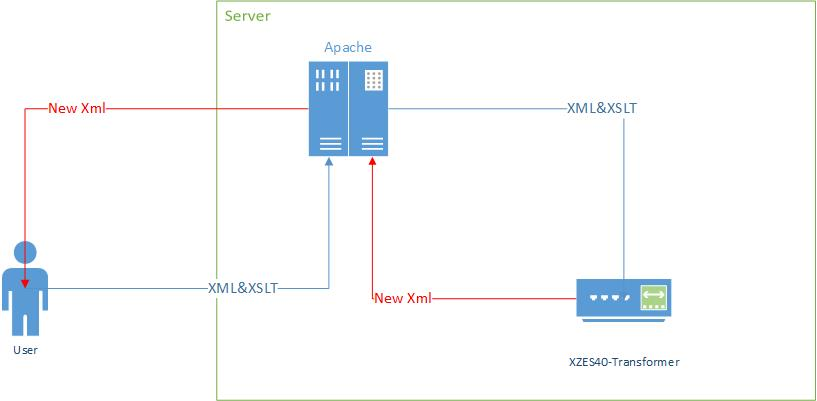
\includegraphics[width=0.5\textwidth]{figures/document-flow-digram}
  \caption{
    Diagram of dataflow.
    Documents are sent to the application through the Apache gateway interface.
    Once processed documents are returned to the user through the gateway interface again.
  }
\end{figure}
        
\begin{figure}[hp]
  \centering
  \captionsetup{justification=centering,margin=2cm}
  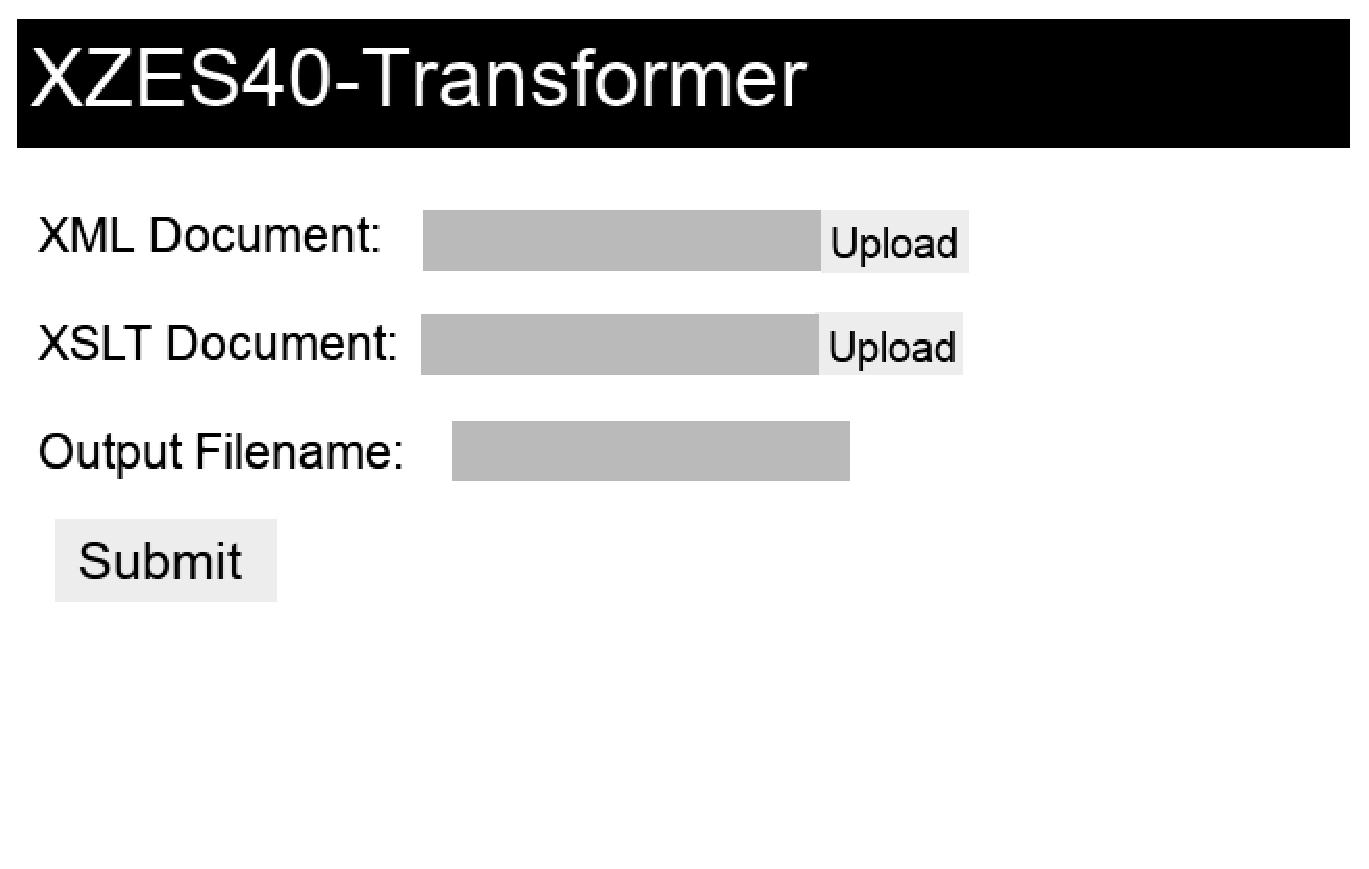
\includegraphics[width=0.5\textwidth]{figures/website-raw}
  \caption{
    Prototype of the Web Interface.
    Demonstrates the simplicity of the interface and required form fields.
  }
\end{figure}

\begin{figure}[hp]
  \centering
  \captionsetup{justification=centering,margin=2cm}
  \begin{lstlisting}
Normal usage:
$ xzes40cli --xml-file='./my-file.xml' --xslt-file='./my-other-file.xslt' --server='http://example.com/xzes40-transformer' --output-file='./newfile.xml' --port='8001'
Sending XML and XSLT files to http:/example.com:8001/xzes40-transformer
Transformation complete. Downloading response file to newfile.xml

Sending a bad file:
$ xzes40cli --xml-file='./badfile.jpg' --xslt-file='./badfile.txt' --server='http://example.com/xzes40-transformer'
Sending XML and XSLT files to http:/example.com:80/xzes40-transformer
ERROR: Server was unable to transform the requested files.

Using inadequate parameters
$ xzes40cli
Please provide an xml file (--xml-file), xslt file (--xslt-file) and a host (--server).
  \end{lstlisting}
  \caption{Example use-cases of CLI interface.}
\end{figure}

\begin{figure}[hp]
  \centering
  \captionsetup{justification=centering,margin=2cm}
  \begin{PstGanttChart}[yunit=1,
                        xunit=1,
                        ChartUnitIntervalName=W,
                        ChartUnitBasicIntervalName=W,
                        TaskUnitIntervalValue=10,
                        TaskUnitType=W,
                        ChartStartInterval=1,
                        ChartShowIntervals]{20}{19}
   \psset{gradangle=180}
   \PstGanttTask[TaskStyle=Important,TaskInsideLabel={Alpha}]{0}{6}
   \PstGanttTask[TaskInsideLabel={Benchmark Data Collection}]{0}{3}
   \PstGanttTask[TaskInsideLabel={Core Functionality}]{0}{11}
   \PstGanttTask[TaskInsideLabel={Basic Transformation}]{0}{3}
   \PstGanttTask[TaskInsideLabel={Caching}]{3}{7}
   \PstGanttTask[TaskInsideLabel={Parallel Computation}]{3}{7}
   \PstGanttTask[TaskInsideLabel={Demo}]{5}{1}
   \PstGanttTask[TaskStyle=Important,TaskInsideLabel={Beta}]{6}{5}
   \PstGanttTask[TaskInsideLabel={CGI Script}]{7}{1}
   \PstGanttTask[TaskInsideLabel={Web Interface}]{8}{2}
   \PstGanttTask[TaskInsideLabel={Debian Package}]{9}{2}
   \PstGanttTask[TaskInsideLabel={Demo}]{10}{1}
   \PstGanttTask[TaskStyle=Important,TaskInsideLabel={Release}]{12}{7}
   \PstGanttTask[TaskInsideLabel={CLI Interface}]{12}{2}
   \PstGanttTask[TaskInsideLabel={RedHat Package}]{12}{6}
   \PstGanttTask[TaskInsideLabel={BSD Package}]{12}{6}
   \PstGanttTask[TaskInsideLabel={Windows Package}]{12}{6}
   \PstGanttTask[TaskInsideLabel={Demo}]{17}{2}
   \PstGanttTask[TaskStyle=NotImportant]{11}{1}
  \end{PstGanttChart}
  \caption{Development Gantt Chart Timeline.}
\end{figure}


\subsection{Added requirements}
%%%%%%%%%%%%%%%%%%%%%%%%%%%%%%%%%%%%%%%%%%%%%%%%%%%%%%%%%%%%%%%%%%%%%%%%%%%%%%%%
% What new requirements were added?
% Why?
% Use the following table format:
% | 1 | Requirement | What happened to it | Comments
% | 2 | Requirement | What happened to it | Comments
% | 3 | Requirement | What happened to it | Comments
%%%%%%%%%%%%%%%%%%%%%%%%%%%%%%%%%%%%%%%%%%%%%%%%%%%%%%%%%%%%%%%%%%%%%%%%%%%%%%%%

This section outlines requirements added to the project during development.

\begin{table}[H]
  \begin{center}
    \begin{tabular}{ | c | c | p{7cm} | p{6cm} | }
      \hline 
      \# & Requirements & What happened & Comments \\ \hline
      1 & Parameter passing & This is a simple parameter passing requirement that is required by client in spring term. It just pass the parameter to our transformer, so transformer know what the output looks like & \\ \hline
      2 & Additional file passing & Some XML file and XSLT file require the DTD file which is a database file, so we add this function to our transformer, because we need benchmark our program.& \\ \hline
    \end{tabular}
  \end{center}
  \caption{Added requirements and rationales.}
\end{table}

\subsection{Updated requirements}
%%%%%%%%%%%%%%%%%%%%%%%%%%%%%%%%%%%%%%%%%%%%%%%%%%%%%%%%%%%%%%%%%%%%%%%%%%%%%%%%
% What existing requirements were changed?
% Why?
% Use the following table format:
% | 1 | Requirement | What happened to it | Comments
% | 2 | Requirement | What happened to it | Comments
% | 3 | Requirement | What happened to it | Comments
%%%%%%%%%%%%%%%%%%%%%%%%%%%%%%%%%%%%%%%%%%%%%%%%%%%%%%%%%%%%%%%%%%%%%%%%%%%%%%%%

This section outlines requirements which changed during development.

\begin{table}[H]
  \begin{center}
    \begin{tabular}{ | c | c | p{7cm} | p{6cm} | }
      \hline
      \# & Requirements & What happened & Comments \\ \hline
      1 & Daemon & This requirement was more complex than initially expected, there was confusion about the complexity of this component. We were originally unclear about weather we needed to run a daemon for our in-memory cache, or if we could store the cache in a separate application like Redis. & \\ \hline
      2 & CLI Interface & A CLI Interface was not explicitly created for the application, however one was created for testing purposes. & With small changes this interface may be created if further development takes place \\ \hline
    \end{tabular}
  \end{center}
  \caption{Updated requirements and rationales.}
\end{table}

\subsection{Removed requirements}
%%%%%%%%%%%%%%%%%%%%%%%%%%%%%%%%%%%%%%%%%%%%%%%%%%%%%%%%%%%%%%%%%%%%%%%%%%%%%%%%
% What existing requirements were deleted?
% Why?
% Use the following table format:
% | 1 | Requirement | What happened to it | Comments
% | 2 | Requirement | What happened to it | Comments
% | 3 | Requirement | What happened to it | Comments
%%%%%%%%%%%%%%%%%%%%%%%%%%%%%%%%%%%%%%%%%%%%%%%%%%%%%%%%%%%%%%%%%%%%%%%%%%%%%%%%

This section outlines requirements which were removed during development.

\begin{table}[H]
  \begin{center}
    \begin{tabular}{ | c | c | p{7cm} | p{6cm} | }
      \hline
      \# & Requirements & What happened & Comments \\ \hline
      1 & Installation Package &
        This requirement was not explicitly removed from the requirements list, however no effort was made to complete this component of the project. & 
        Neither the core requirements, a Debian package, nor the stretch goals, a Windows, CentOS, and BSD package, were pursued.
        The client agreed that as a prototype an installation package was not required to call the project as success. \\ \hline
      2 & Mutilate platform  &
        This is a strength goal for our requirements, but we consider to remove it, because some technology that we used is heavy based on the Linux system.
    \end{tabular}
  \end{center}
  \caption{Removed requirements and rationales.}
\end{table}
